\documentclass{beamer}
%\documentclass[handout]{beamer}

\usetheme{AlbaSynchrotron}

\usepackage[utf8]{inputenc}
\usepackage{default}
\usepackage{hyperref}
\usepackage[absolute,overlay]{textpos}
\usepackage{graphicx}
\usepackage{listings}

\usefonttheme[onlymath]{serif}

\title[Skippy]
  {Python Device server for SCPI instruments}
%\subtitle{Standard Commands for Programmable Instruments}

\author[Sergi Blanch-Torn\'e] % (optional, for multiple authors)
{S.~Blanch-Torn\'e\inst{1} \and A.~Mil\'an\inst{2} \and M.~Broseta\inst{1} \and C.~Falc\'on\inst{1} \and J.~Andreu\inst{1} \and D.~Rold\'an\inst{1} \and J.~Moldes\inst{1} \and G.~Cun\'{\i}\inst{1}}
\institute[ALBA Synchrotron] % (optional)
{
  \inst{1}%
  ALBA Synchrotron, CELLS\\
  Cerdanyola del Vall\`es
  \and
  \inst{2}%
  MAX IV Laboratory\\
  Lund
}
\date[Hamburg 2019] % (optional)
{Tango Meeting, 2019}
\subject{Tango Devices}

\begin{document}

\frame{\titlepage}

\begin{frame}
\frametitle{Table of Contents}
\tableofcontents%[currentsection]
\end{frame}

% \AtBeginSection[]
% {
%   \begin{frame}
%     \frametitle{Table of Contents}
%     \tableofcontents[currentsection]
%   \end{frame}
% }
% 
% \AtBeginSubsection[]
% {
%   \begin{frame}
%     \frametitle{Table of Contents}
%     \tableofcontents[currentsection,currentsubsection]
%   \end{frame}
% }

\section{What's SCPI?}

\begin{frame}
  \frametitle{What's \href{https://en.wikipedia.org/wiki/Standard_Commands_for_Programmable_Instruments}{SCPI}?}
  \framesubtitle{Standard Commands for Programmable Instruments}
  \begin{block}{From the \href{https://en.wikipedia.org/wiki/Standard_Commands_for_Programmable_Instruments}{wikipedia}'s definition}<+->
    The \emph{Standard Commands for Programmable Instruments} (SCPI; often pronounced "skippy") defines a standard for syntax and commands to use in controlling programmable test and measurement devices, such as automatic test equipment and electronic test equipment.
  \end{block}
  \begin{alertblock}{Standard definition}<+->
    \begin{itemize}
      \item \textcolor{AlbaBlue}{\href{http://www.ivifoundation.org/docs/scpi-99.pdf}{SCPI-99}}
      \item \textcolor{AlbaBlue}{\href{http://dx.doi.org/10.1109/IEEESTD.2004.95390}{IEEE 488.2-2004}}
    \end{itemize}
  \end{alertblock}
  \begin{exampleblock}{How it looks like:}<+->
    \begin{columns}
      \begin{column}{0.18\textwidth}
        {\tt *IDN?},\\
        {\tt *RST},...
      \end{column}
      \begin{column}{0.60\textwidth}
	\textcolor{AlbaBlue}{{\tt SOURce:FREQuency:STARt?}, \\{\tt SYSTem:COMMunicate:SERial:BAUD 2400}}
      \end{column}
    \end{columns}
  \end{exampleblock}
\end{frame}
  
\section{Tango Device Servers}

\begin{frame}
  \frametitle{Tango Device Servers}
  \framesubtitle{What we (all) did with SCPI, or at least what I've seen:}
  \begin{itemize}
    \item<+-> At least 49 Device Servers identified in the Catalogue
    \item<+-> Represents $>$ 6\% of the current Device Servers in the inventory
    \item<+-> 40 are written in Cpp, 8 in Python, 1 in Java
  \end{itemize}
  \begin{columns}
    \begin{column}{0.45\textwidth}
      \begin{exampleblock}{by Family}<+->
         \begin{tabular}{lr}
           Communications          &  8 \\
           Instrumentation         & 19 \\
           Measurement Instruments & 20 \\
           Other Instruments       &  1 \\
           Standard Interfaces     &  1 \\
         \end{tabular}
      \end{exampleblock}
    \end{column}
    \begin{column}{0.45\textwidth}
      \begin{exampleblock}{by Institute}<+->
          \begin{tabular}{lr}
            3control & 1\footnote{\href{https://www.tango-controls.org/developers/dsc/ds/1508/}{ScpiDS} multiple instruments} \\
            alba & 7 \\
            desy & 22 \\
            esrf & 8 \\
            nexeya & 2 \\
            soleil & 9 \\
          \end{tabular}
      \end{exampleblock}
    \end{column}
  \end{columns}
  \begin{textblock*}{75pt}(265pt,150pt)
    \begin{alertblock}{Skippy:}<+->
      13 instruments\\
      9 manufacturers\\
      4 in progress
    \end{alertblock}
  \end{textblock*}
\end{frame}

\subsection{SkippyDS}

\begin{frame}
  \frametitle{\href{https://www.tango-controls.org/developers/dsc/ds/2376/}{SkippyDS}}
  \framesubtitle{State machine and tango description}
  \begin{textblock*}{270pt}(20pt,40pt)
  \centering{
    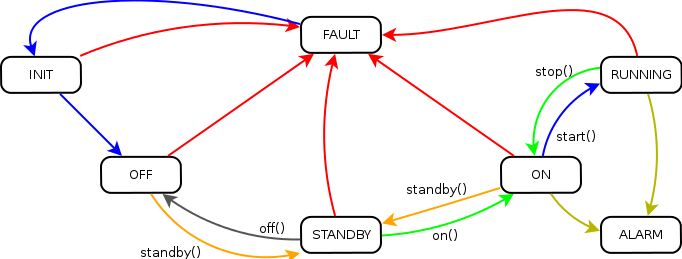
\includegraphics[keepaspectratio=true,width=0.9\columnwidth]{../StateMachine.png}
  }
  \end{textblock*}
  \begin{textblock*}{180pt}(30pt,130pt)
    \begin{block}{commands}<2->
      \begin{itemize}
        \item {\tt IDN()}
        \item {\tt Off(), Standby(), On()}
        \item {\tt Start(), Stop()}
        \item {\tt \{Add,Remove\}Monitoring()}
        \item {\tt \{Get,Set\}MonitoringPeriod()}
        \item {\tt CMD()}
      \end{itemize}
    \end{block}
  \end{textblock*}
  \begin{textblock*}{140pt}(210pt,165pt)
    \begin{block}{attributes}<3->
      \begin{itemize}
        \item {\tt QueryWindow}
        \item {\tt TimeStampsThreshold}
      \end{itemize}
    \end{block}
  \end{textblock*}
  \begin{textblock*}{210pt}(130pt,30pt)
    \begin{block}{Properties}<4->
      \begin{itemize}
        \item {\tt Instrument}
        \item {\tt Port}
        \item {\tt Serial\{Baudrate,Bytesize,...\}}
        \item {\tt Num\{Channels,Functions,Multiple\}}
        \item {\tt MonitoredAttributes}
        \item {\tt Auto\{Standby,On,Start\}}
        \item {\tt TxTerminator}
      \end{itemize}
    \end{block}
  \end{textblock*}
\end{frame}

\begin{frame}
  \frametitle{\href{https://www.tango-controls.org/developers/dsc/ds/2376/}{SkippyDS}}
  \framesubtitle{How to define an attribute?}
  \begin{exampleblock}{Attribute builder}
    \lstinputlisting[language=Python, basicstyle=\ttfamily\tiny]{attrBuilder.py}
  \end{exampleblock}
  \begin{block}{keywords}
     \begin{columns}
       \begin{column}{0.40\textwidth}
         \begin{itemize}
           \item {\tt type}, {\tt dim}
           \item {\tt label}, {\tt description}, 
           \item {\tt format}, {\tt unit}, 
           \item {\tt memorized}
           \item {\tt min/max}
         \end{itemize}
       \end{column}
       \begin{column}{0.40\textwidth}
         \begin{itemize}
           \item {\tt readCmd},  {\tt writeCmd}
           \item {\tt channels}, {\tt functions}, {\tt multiple}
           \item {\tt delayAfterWrite}
           \item {\tt readFormula}
         \end{itemize}
       \end{column}
     \end{columns}
  \end{block}
\end{frame}

\begin{frame}
  \frametitle{Instrument builder}
  %\framesubtitle{Software patterns}
  \centering{
    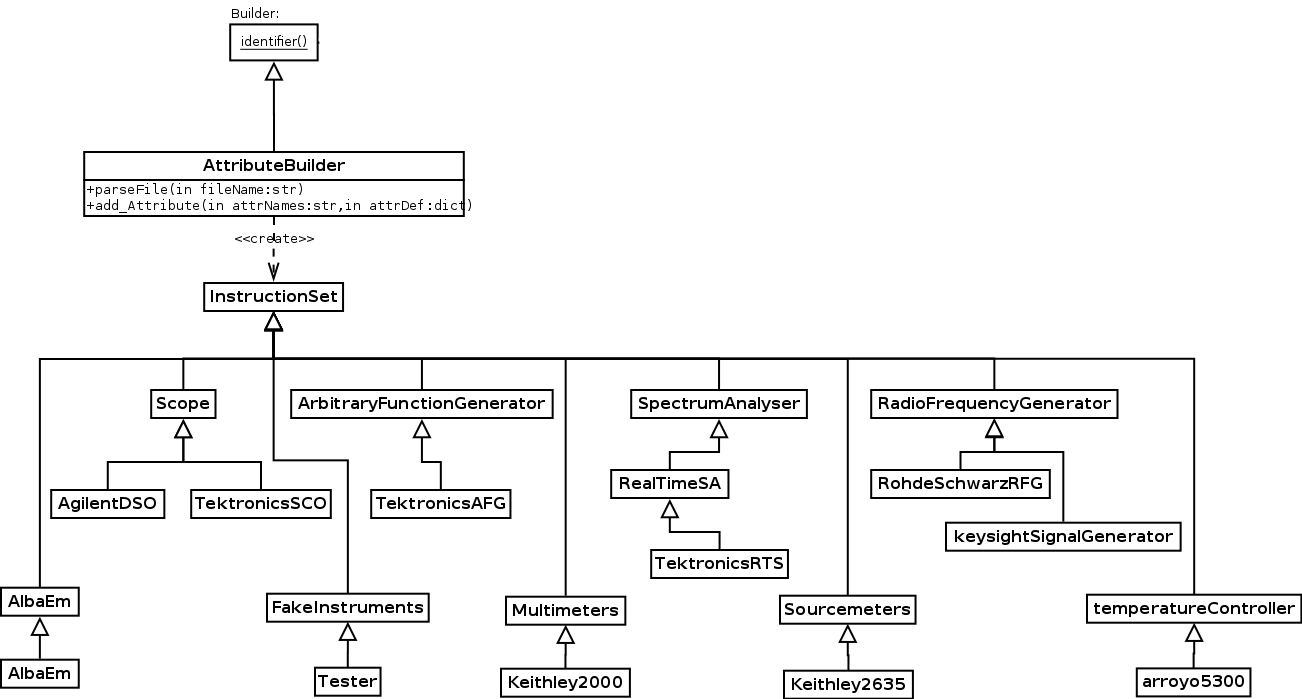
\includegraphics[keepaspectratio=true,width=0.7\paperwidth]{Builder.png}
  }
\end{frame}

\begin{frame}
  \frametitle{Instrument requests}
  \centering{
    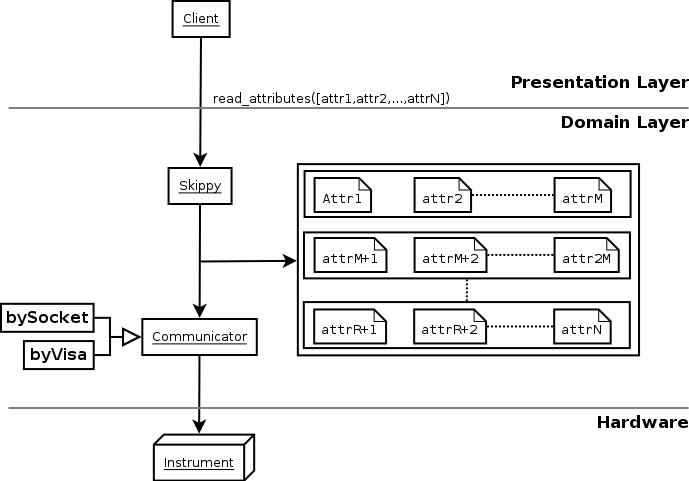
\includegraphics[keepaspectratio=true,width=0.7\paperwidth]{../groupedRequests.png}
  }
\end{frame}

\subsection{Sardana Controller}

\begin{frame}
  \frametitle{Sardana Controller}
  \begin{enumerate}
    \item<2-> Use a proxy in the controller
    \item<3-> Reduce layers: Instead of use a tango device, implement a native access to the instruments in the controller
  \end{enumerate}
  \begin{itemize}
    \item<4-> \alert{Again}, one specific controller per instrument?
    \item<5-> \alert{Reimplement} generic features?
    \item<6-> {\color{green}Encapsulate and share} the features: a python module
  \end{itemize}
\end{frame}

\section{Python module}

\subsection{python-skippy}

\begin{frame}
  \frametitle{python-skippy module}
  \centering{
    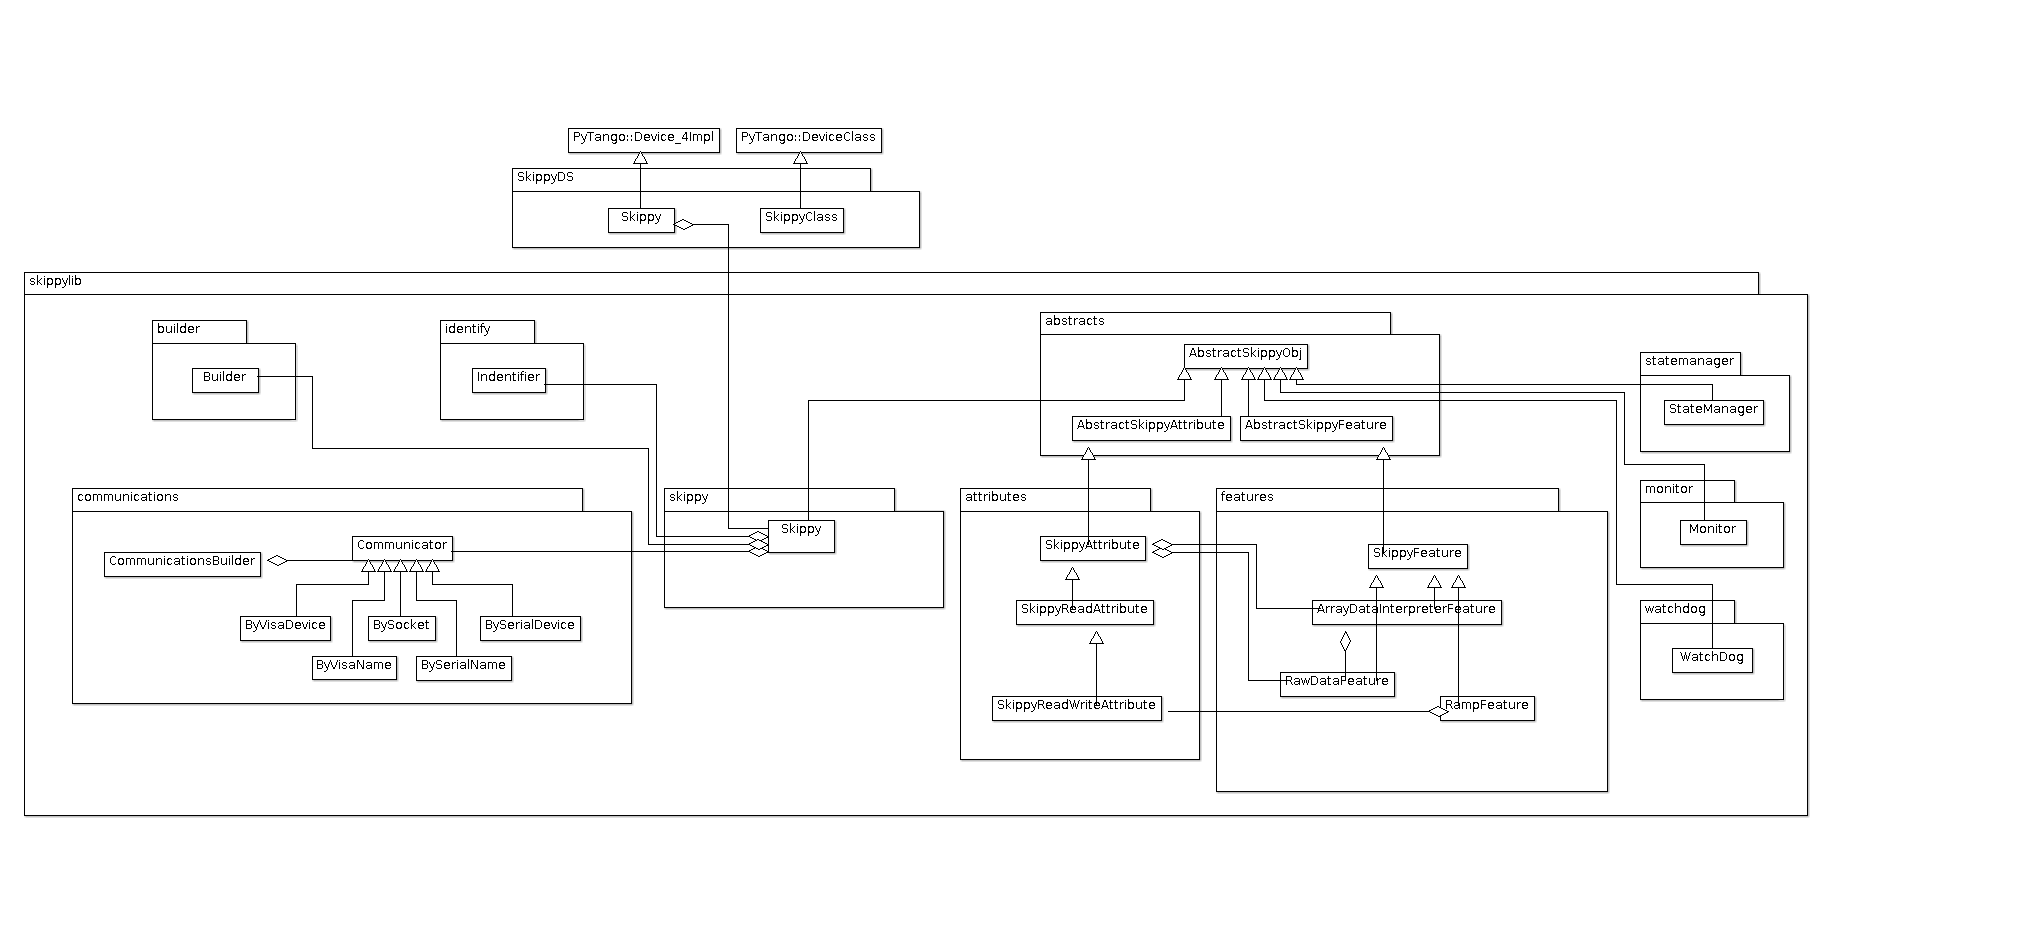
\includegraphics[keepaspectratio=true,width=1\paperwidth]{SkippyGeneralClassDiagram.png}
  }
  \begin{textblock*}{160pt}(10pt,200pt)
    \begin{block}{{\tiny Software patterns}}
      \begin{itemize}%[itemindent=0pt]
        \setlength{\itemsep}{-7pt}
        \setlength{\parskip}{0pt}
        \setlength{\parsep}{-5pt}
        \item[] {\tiny Strategy pattern on the communications} \\
        \item[] {\tiny Singleton on statemanager, monitor and watchdog} \\
        \item[] {\tiny Composite in the attributes}
      \end{itemize}
    \end{block}
  \end{textblock*}
  \begin{textblock*}{260pt}(60pt,60pt)
    \begin{exampleblock}{Python console example}<2->
      \lstinputlisting[language=Python, basicstyle=\ttfamily\tiny]{skippyObj.py}
    \end{exampleblock}
  \end{textblock*}
\end{frame}

\begin{frame}
  \frametitle{In practice @ ALBA}
  \begin{itemize}
    \item<2-> Master oscillator
    \begin{itemize}
      \item Radiofrequency generator
    \end{itemize}
    \item<3-> Measured Filling Pattern: 
    \begin{itemize}
      \item Oscilloscope with the filling pattern
      \item Many Oscilloscopes in the accelerator with we can cross different source signals
    \end{itemize}
    \item<4-> Tune excitation:
    \begin{itemize}
      \item Arbitrary Function Generator
      \item Spectrum analyzer
    \end{itemize}
    \item<5-> Beamline \& Laboratory instruments
    \begin{itemize}
      \item Source \& Multimeters
      \item Pump controller \only<5->{\footnote{LN2 pump where J.Andreu has had to write the server side scpi in C\#}}
      \item Temperature controller \only<5->{\footnote{It doesn't work as scpi but string-like protocol}}
    \end{itemize}
    \item<6-> Alba \#Em \& Music SiPM
    \begin{itemize}
      \item We close the circle with the scpilib
    \end{itemize}
  \end{itemize}
\end{frame}


\subsection{python-scpilib}

\begin{frame}
  \frametitle{python-scpilib module}
  \centering{
    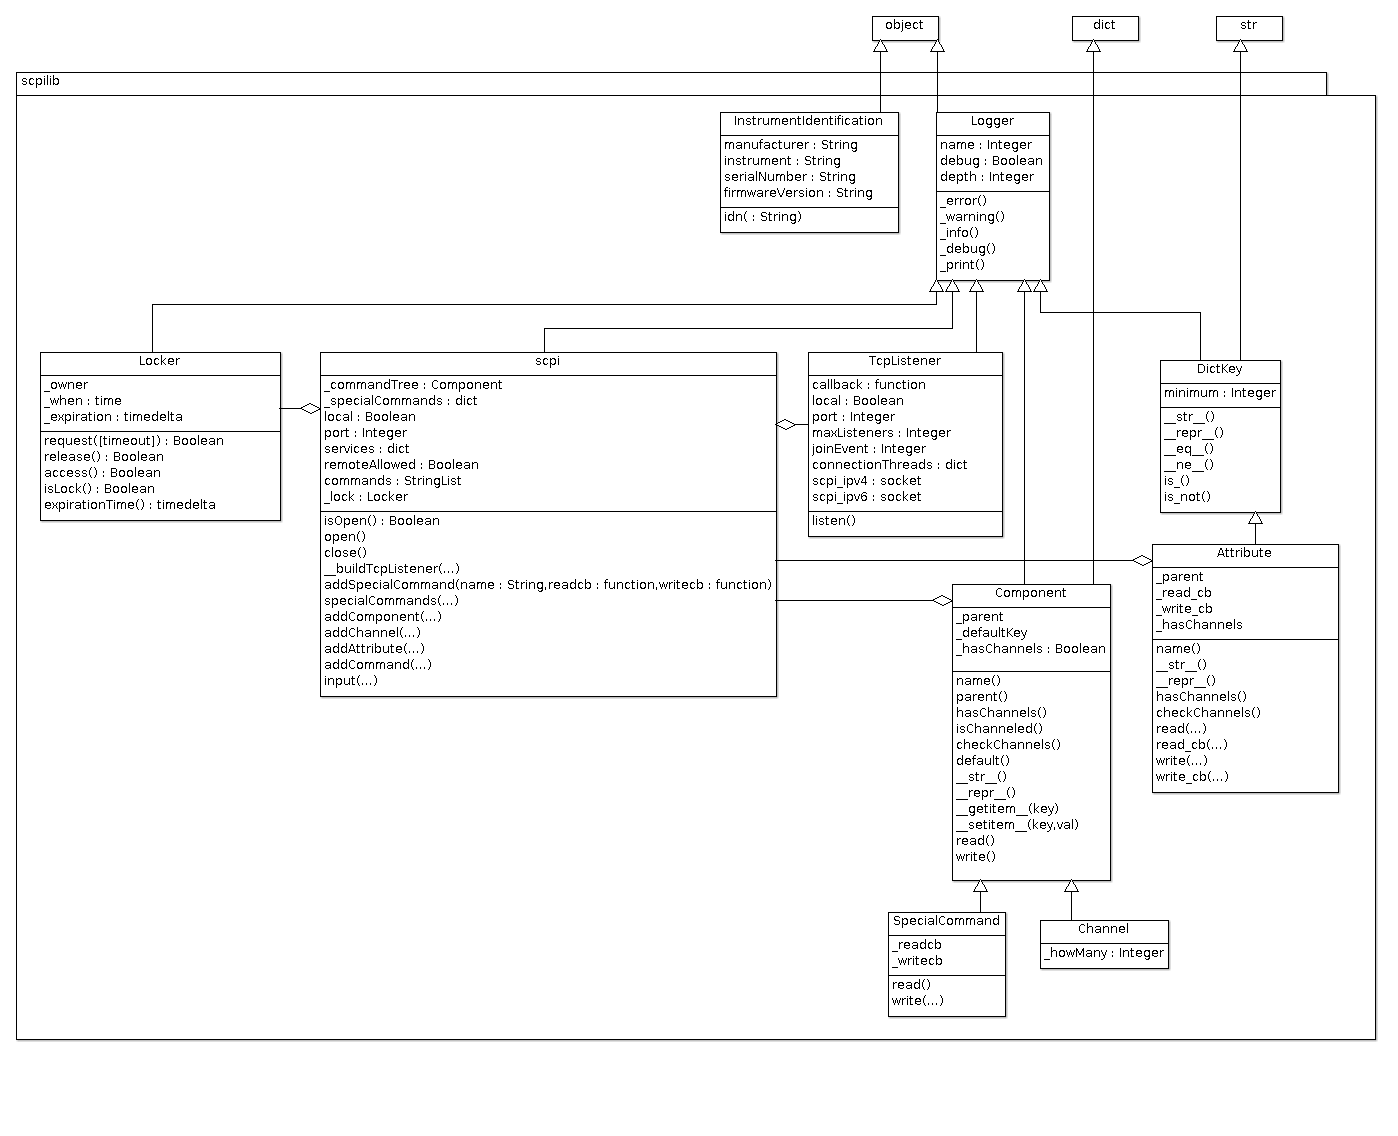
\includegraphics[keepaspectratio=true,width=0.8\paperwidth]{ScpilibClassDiagram.png}
  }
\end{frame}

\section{Wish \& ToDo lists}

\begin{frame}
  \frametitle{Wish \& ToDo Lists}
  \begin{textblock*}{0.45\textwidth}(30pt,25pt)
    \begin{block}{skippylib}<2->
      \begin{itemize}
        \item<alert@3> Improve new instrument insertion
        \item Improve the watchdog
        \item Dynamic attributes as property
        \item Dynamic commands
        \item Generalize \emph{TxTerminator}
        \item Different ramp strategies
        \item {\tt WriteFormula}
        \item input validation
        \item dependencies with state-like
      \end{itemize}
    \end{block}
  \end{textblock*}
  \begin{textblock*}{0.45\textwidth}(200pt,25pt)
    \begin{exampleblock}{scpilib}<4->%https://github.com/srgblnch/python-scpilib#features-requested-wishtodo-list
      \begin{itemize}
        \item<alert@5> \emph{autodoc} scpi tree
        \item<alert@6> python3
        \item Set of \emph{minimal} commands
        \item Write lock (current is RW)
        \item Report locker owner
        \item Extend \emph{lock} feature to subtrees
        \item Listen more channels than network
        \item SSL and ACLs
        \item Event subscription
        \item multidimensional data
      \end{itemize}
    \end{exampleblock}
  \end{textblock*}
  \begin{textblock*}{0.7\textwidth}(10pt,220pt)
    \begin{alertblock}{gui}<7->
       \begin{itemize}
         \item Generic \href{www.taurus-scada.org}{taurus} gui for any of the instruments
       \end{itemize}
    \end{alertblock}
  \end{textblock*}
\end{frame}

\end{document}
